\documentclass[11pt, oneside]{article}  

\usepackage{style-3yp} %this is the .sty file
\usepackage{pdflscape}
\lfoot{Enzia Schnyder} %your name in the footer

\usepackage{float}
\usepackage{longtable}
%table
\usepackage{array}
\newcolumntype{L}{>{\centering\arraybackslash}m{2.5cm}}
\newcolumntype{J}{>{\centering\arraybackslash}m{4.1cm}}
\newcolumntype{M}{>{\centering\arraybackslash}m{5cm}}
\newcolumntype{N}{>{\centering\arraybackslash}m{3.5cm}}
\usepackage{multirow}

\usepackage{gensymb} %degrees symbol
\usepackage [version=4] {mhchem}


\begin{document}
\section{Gas Turbine}

\begin{table} [h]
\begin{center}
\caption{Properties of the ammonia-air mixture. Lower and upper flammability limits (LFL \& UFL) are measured by volume percentage of air \cite{FL}} \label{tab:mixproperties}
\begin{tabular}{ |c|c|c|c|c|c| }
 \hline
& Mr (a.m.u) & LCV (MJ/kg) \cite{website:spg}& LCV (MJ/kmol) & LFL (\%)& UFL (\%) \\ 
 \hline
  $H_2$ & 2.02 & 120.1 & 242.6 & 4.0 & 75.0\\ 
 \hline
$NH_3$ & 17.03 & 18.6 & 316.8 & 15.0 & 28.0\\ 
 \hline
$H_2/NH_3$ mixture & 10 & 28.6 & 334.7 & 6.47 & 40\\
 \hline
\end{tabular}
\end{center} 
\end{table}

\begin{figure} [h]
\centering
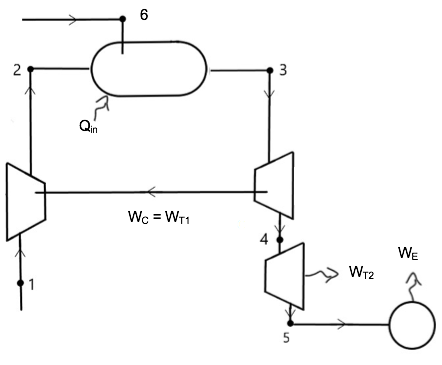
\includegraphics[width=0.58\textwidth]{./pictures/plantdiagram.png}
  \caption{The turbine diagram, showing all streams, work inputs, outputs and heat inputs} \label{fig:turbinediagram}
  \end{figure}
  
  \begin {table} [h]
\begin{center}
\caption{Heat inputs and work outputs of the system} \label{tab:powerdata} 
\begin{tabular}{ |c|c| }
 \hline
  $W_{T1}$ & 80.9MW\\ 
 \hline
  $W_{T2}$ & 89.3MW\\
  \hline
  $W_E$ & 723.6kW\\
 \hline
 $Q_{in}$ & 210.5MW\\
 \hline
 Overall Efficiency & 0.6423\\ 
 \hline
\end{tabular}
\end{center}  
\end {table}

\newpage

\section{Heat Exchange Network}
\begin{figure} [h]
\centering
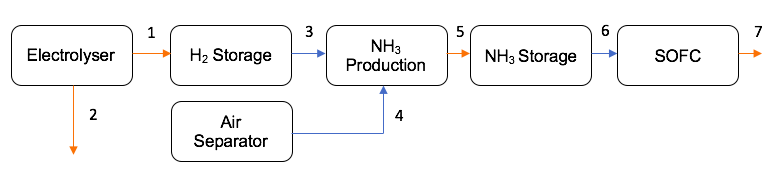
\includegraphics[width=0.9\textwidth]{./pictures/heatexflow.png}
  \caption{A diagram showing how different streams in the heat exchange network are related to the process units. Blue arrows represent cold streams that must be heated up and red arrows represent hot streams that must be cooled} \label{fig:heatexflow}
\end{figure}

\begin{table} [h]
\begin{center}
\caption{Data for streams coming in and out of all major process units of the ESS plant} \label{tab:heatexdata} 
\begin{tabular}{ |c|c|L|c|c|c|L| }
 \hline
Stream & Composition & $\dot{m} $ $(kg/s) $& $C_p$ $(kJ kg^{-1} K^{-1})$  & $T_{in}$ $(K)$ & $T_{out}$ $(K)$ & $\Delta H$ $(kW)$ \\ 
 \hline
  1 & $H_2$ & 0.4844 & 14.3 & 393 & 298 & -658\\ 
 \hline
 2 & $O_2$ & 35.75 & 0.919 & 393 & 298 & -3119\\ 
 \hline
3 & $H_2$ & 0.5099 & 14.3 & 298 & 473 & 1276\\
\hline
4 & $N_2$ & 2.34 & 1.04 & 288 & 473 & 450.2\\
 \hline
  5 & $NH_3$ & 2.795 & 2.19 & 238 & 233 &-30.6\\
 \hline
 6 & $NH_3$ & 2.655 & 2.19 & 233 & 243 & 58.1\\
 \hline
 7 & Air & 500 & 1.01 & 898 & 298 & -303000\\
 \hline
\end{tabular}
\end{center}  
\end{table}

\begin{figure} [H]
\centering
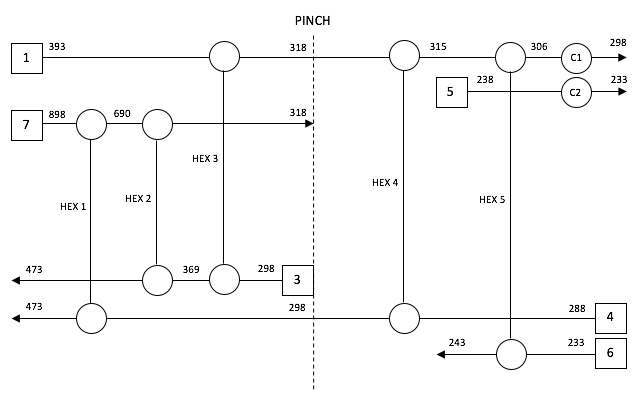
\includegraphics[width=0.72\textwidth]{./pictures/heatexnetwork.png}
  \caption{The final heat exchange network. Each pair of circles represents a heat exchanger, single circles represent cooling utility and temperatures (K) are shown at each isothermal segment.} \label{fig:heatexnetwork}
  \end{figure}

\begin {table} [h]
\begin{center}
\caption{Heat transferred in all heat exchangers and utilities in the network} \label{tab:powerhex} 
\begin{tabular}{ |c|c|c|c|c|c|c|c|c| }
 \hline
\multirow{2}{*}{Component} & \multicolumn{5}{|c|}{Heat exchangers }& \multicolumn{2}{|c|}{Cooling Utilities}\\ 
 \cline{2-8}
   & HEX 1 & HEX 2 & HEX 3 & HEX 4 &HEX 5 & C1 & C2\\ 
 \hline
 Enthalpy change (kW) & 425.3 & 756.0 & 519.8 & 24.3 & 58.1 & 56.2 & 30.6\\ 
 \hline
\end{tabular}
\end{center}  
\end {table}
\end{document}
